\documentclass[11pt,a4paper]{article}
\usepackage[margin=24mm]{geometry}
\usepackage[T1]{fontenc}
\usepackage{lmodern,booktabs,tabularx,graphicx,amsmath,xcolor}
\usepackage[hidelinks]{hyperref}
\usepackage{microtype}
\definecolor{teal}{HTML}{087F75}
\usepackage{titlesec}
\titleformat{\section}{\large\bfseries\color{teal}}{\thesection}{1em}{}
\setlength{\parindent}{0pt}
\setlength{\parskip}{6pt}
\setlength{\emergencystretch}{2em}
\title{\textbf{HiggsLens}\\Particle Event Classification via Expert Features\\and Neural Networks}
\author{Saumya Mishra \and Aditya Rana \and Rachit Gupta \and Ronit Singh \and Krishna}
\date{Project 10 --- Research and Evidence Review\\17 November 2026}
\begin{document}
\maketitle
\begin{abstract}
We review a reproducible benchmark for classifying simulated UCI HIGGS events, comparing Logistic Regression and XGBoost with compact, deep and residual multilayer perceptrons. The required course experiment is the compact MLP against classical baselines at a fixed data budget. Deeper models are extensions testing representation capacity. Saved release summaries cover three feature groups at 250,000, one million and 2.5 million events. At 2.5 million events with all features, the recorded residual MLP achieves ROC-AUC 0.8613 versus 0.8382 for XGBoost, with greater training cost and worse expected calibration error. These are single-seed benchmark observations, not universal model rankings or discovery claims. A fresh audit recomputed three metrics for all 15 published 250,000-event prediction files; larger-budget summaries were inspected but their predictions and original training data are absent locally. We distinguish verified artifacts, literature motivation and proposed follow-up experiments throughout.
\end{abstract}
\begingroup\small\setlength{\parskip}{0pt}\tableofcontents\endgroup
\newpage
\section{Problem and alignment with the course brief}
The target is binary event classification: signal versus background in Monte Carlo simulations. The output is a classifier score, not a statement that a real particle was detected. UCI provides 11 million events with 21 low-level numerical features and seven expert-derived high-level features \cite{uci,baldi}. The source file's row count must not be presented as the number of events used in every training run.

The hybrid logic is a comparison between expert representations and learned numerical interactions. It does not imply a stacked tree--neural hybrid or an ensemble. Logistic Regression supplies an interpretable linear reference; XGBoost provides a nonlinear tabular baseline; the compact MLP tests learned interactions on the same inputs. Compare low-level, high-level and combined representations under the same split. Required outcomes are discrimination, calibration and compute trade-offs at a documented subset budget before scaling.

\begin{tabularx}{\linewidth}{@{}lX@{}}\toprule
Brief requirement & Review of current implementation\\\midrule
Classical baselines & Logistic Regression and XGBoost implemented across three groups.\\
Compact MLP & Implemented with BatchNorm, dropout and validation stopping.\\
Fixed-budget evaluation & Shared split within each budget; 250k is the starter benchmark.\\
Stratified subset & Release subset selection uses a seeded random permutation; the subsequent split is stratified. Explicit stratified subset sampling remains a gap.\\
Memory-safe loading & The data library has chunked readers; the release runner materializes the full raw array to deduplicate before sampling.\\
Standardized inputs & Logistic Regression and MLP scale training-only. XGBoost takes unscaled numeric inputs; document this deviation from the brief or add a controlled scaled-input run.\\
Scaling & 1M and 2.5M summaries exist; the test population changes across budgets.\\\bottomrule
\end{tabularx}

\section{Why investigate deep learning after XGBoost?}
Baldi et al. motivate representation learning for high-energy physics: nonlinear networks can extract useful interactions from low-level measurements and reduce dependence on manually engineered features \cite{baldi}. This is a reason to test deeper models, not proof that any neural implementation will win.

XGBoost is a scalable, regularized boosted-tree system \cite{xgboost}. It must remain a strong comparison, especially when compute or probability calibration matters. Broader tabular benchmarks find trees highly competitive, including on medium-sized datasets; those findings do not automatically transfer to this much larger physics benchmark \cite{grinsztajn}. Gorishniy et al. motivate residual MLP and feature-token Transformer comparisons while finding no universally superior model \cite{gorishniy}.

Glorot and Bengio explain how activation saturation and initialization can affect optimization in deep networks \cite{glorot}. This supports discussing gradient flow, initialization and training diagnostics. It is not evidence that the present code explicitly uses Xavier initialization: the implementation relies on PyTorch layer defaults and does not implement the paper's initialization procedure.

At 250k events and a fixed score cutoff of 0.5, all-feature test accuracy is 73.75\% for XGBoost, 74.70\% for Deep MLP and 75.26\% for Residual MLP. These gains of 0.95 and 1.51 percentage points are modest and lack repeat-seed uncertainty. Keep Logistic Regression, XGBoost and compact MLP as the core project; treat larger networks as exploratory extensions. Similar accuracy does not mean identical ranking or calibration: accuracy measures one operating point, while AUC evaluates ranking over thresholds. Neither metric should be substituted for the other.

The defensible selection statement is conditional: choose a validated deep model when the measured discrimination gain justifies the compute and calibration costs. Keep XGBoost for a different operating budget. Select hyperparameters and models using validation evidence before reporting the held-out test; do not optimize against the table of test scores.

\section{Models and implementation choices}
Let $D\in\{21,7,28\}$ denote the input dimension. Neural models produce one logit $z(x)$, train with binary cross entropy with logits, and use $\sigma(z)$ as an evaluation score. Standardization is fitted on training rows only.
\begin{itemize}
\item \textbf{Logistic Regression:} standardized inputs, L-BFGS and $C=1$. It tests a linear decision function and establishes whether engineered masses help a simple learner.
\item \textbf{XGBoost:} the release runner sets up to 3,000 trees, depth 8, learning rate 0.1 and validation-log-loss early stopping with patience 50. This is a recorded configuration with early stopping, not documented evidence of a systematic tuning search.
\item \textbf{Compact MLP:} widths 64--32; Linear, BatchNorm, ReLU and dropout 0.20 at each hidden layer. AdamW uses learning rate $10^{-3}$ and weight decay $10^{-4}$; maximum 30 epochs, validation-AUC patience 5.
\item \textbf{Deep MLP:} five 300-unit layers with BatchNorm, ReLU and dropout 0.10. AdamW uses learning rate $10^{-3}$ and weight decay $10^{-5}$, a cosine schedule, maximum 60 epochs and patience 8. Its size is inspired by Baldi et al.; optimizer, activation, regularization, data protocol and training duration differ. Call it an adaptation, not an exact reproduction.
\item \textbf{Residual MLP:} input projection to 256 units and four residual blocks. Each branch uses BatchNorm, expansion to 512, ReLU, dropout, projection to 256 and dropout, with $h_{l+1}=h_l+F(h_l)$. A normalized output head produces one logit. The optimizer and stopping settings match the deep preset.
\end{itemize}
BatchNorm supports optimization; dropout is a regularizer; residual connections create a direct gradient path. These are design motivations, not isolated causal findings from the current experiments. Width, parameter count, optimization and depth change together. A parameter-matched ablation is needed to attribute improvements specifically to depth or residual connections.

\section{Evaluation protocol and evidence boundary}
The release runner removes duplicate full rows before sampling, draws nested seeded sample budgets, then performs a 70/15/15 stratified train/validation/test split at each budget. The summary records 278,698 removed duplicates and zero feature-event overlap between training and test within each budget. These integrity results are recorded outputs; they were not independently reproduced from the absent raw dataset in this review.

All models within a budget use the same indices. Across budgets, the split is recomputed; a smaller-budget test event can therefore become a larger-budget training event. This is not within-budget leakage, but it prevents interpreting the current scaling graph as a fixed-test learning curve. Future scaling should reserve one global test set first, then draw nested stratified training budgets from the remaining pool.

ROC-AUC measures ranking. The repository's ``PR-AUC'' is average precision, rather than trapezoidal integration of the PR curve. Brier score measures squared probability error; ECE here uses 15 equal-width bins and is bin-dependent. Neither calibration metric alone validates deployment probabilities under a different class prevalence. Report training time separately from inference latency, preprocessing, tuning and total wall time.

The original UCI convention holds out the final 500,000 events \cite{uci}; this project's seeded, deduplicated protocol differs. Literature scores should be shown as contextual references, not inserted into the project's leaderboard. AUC does not directly convert to significance: a significance estimate requires event yields, selection, luminosity and systematic/background assumptions. No discovery-significance estimate is made here.

\section{Recorded results}
All tables and the figure below are generated from \texttt{outputs/release/release\_summary.json}. They describe saved runs with seed 42 on a recorded Tesla T4 environment. This review did not retrain those models.
\subsection*{All 28 features: test ROC-AUC}
\begin{center}\begin{tabular}{lrrr}\toprule
Model & 250k & 1M & 2.5M \\\midrule
Logistic Regression & 0.6864 & 0.6838 & 0.6842 \\
XGBoost & 0.8188 & 0.8302 & 0.8382 \\
Compact MLP & 0.8165 & 0.8230 & 0.8255 \\
Deep MLP & 0.8271 & 0.8474 & 0.8591 \\
Residual MLP & 0.8339 & 0.8506 & 0.8613 \\
\bottomrule\end{tabular}\end{center}
\subsection*{21 low-level features: test ROC-AUC}
\begin{center}\begin{tabular}{lrrr}\toprule
Model & 250k & 1M & 2.5M \\\midrule
Logistic Regression & 0.5962 & 0.5939 & 0.5938 \\
XGBoost & 0.7223 & 0.7478 & 0.7669 \\
Compact MLP & 0.7250 & 0.7382 & 0.7448 \\
Deep MLP & 0.7561 & 0.8141 & 0.8396 \\
Residual MLP & 0.7716 & 0.8203 & 0.8532 \\
\bottomrule\end{tabular}\end{center}
\subsection*{2.5M events, all features: trade-offs}
\begin{center}\small\begin{tabular}{lrrrrr}\toprule
Model & ROC-AUC & AP & Brier & ECE & Train (s) \\\midrule
Logistic Regression & 0.6842 & 0.6951 & 0.2222 & 0.0231 & 5.5 \\
XGBoost & 0.8382 & 0.8578 & 0.1632 & 0.0033 & 28.6 \\
Compact MLP & 0.8255 & 0.8465 & 0.1705 & 0.0286 & 124.2 \\
Deep MLP & 0.8591 & 0.8769 & 0.1524 & 0.0156 & 425.5 \\
Residual MLP & 0.8613 & 0.8788 & 0.1513 & 0.0184 & 493.7 \\
\bottomrule\end{tabular}\end{center}

\begin{figure}[htbp]\centering
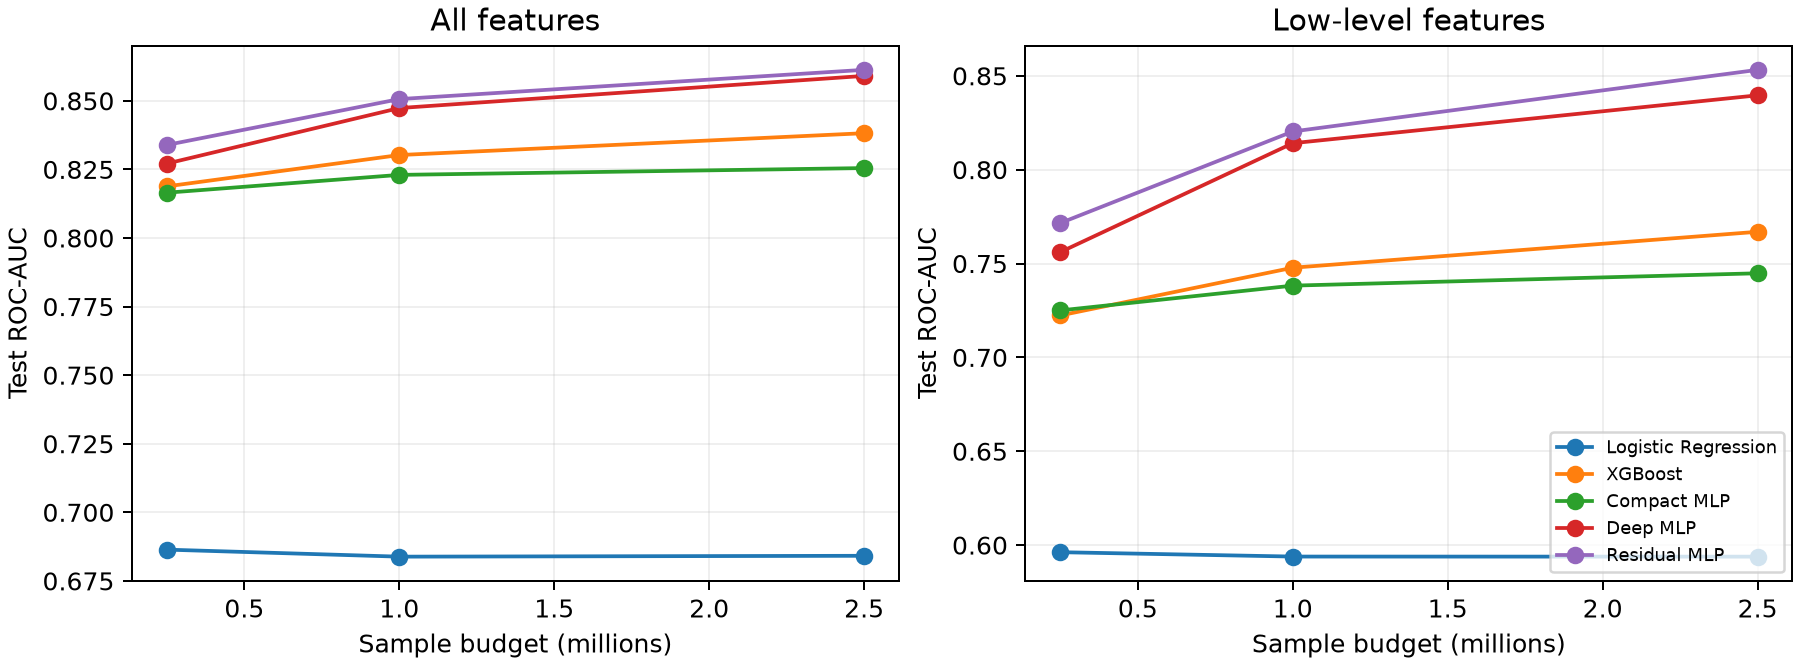
\includegraphics[width=\linewidth]{scaling.png}
\caption{Recorded scaling across sample budgets. Test sets differ between points; lines show descriptive trends, not repeated measurements on one frozen test population.}
\end{figure}

On all features at 2.5M, the residual MLP's ROC-AUC gain over XGBoost is approximately 0.0231. Its training time is about 494 seconds versus 29 seconds (roughly 17 times), and its ECE is 0.0184 versus 0.0033. Thus, the highest recorded ranking performance does not identify a uniformly best model. Residual MLP low-level ROC-AUC 0.8532 exceeds XGBoost all-feature ROC-AUC 0.8382 in this release. This supports the usefulness of learned interactions; it does not prove that hidden units reconstruct the exact invariant-mass formulas.

\section{Fresh audit of saved predictions}
The new audit command is \texttt{python scripts/audit\_saved\_predictions.py}. It checks duplicate row IDs, shared test row IDs and labels, and recomputes ROC-AUC, average precision and Brier score against the saved metric envelopes. All 15 top-level prediction files passed, with 37,500 test events each. The tolerance was $10^{-7}$ absolute, with zero relative tolerance. The machine-readable audit is included in this source bundle.

The 1M and 2.5M directories contain metric envelopes, including training histories, but no test-prediction CSVs in this checkout. Larger-budget numbers are therefore reported summaries rather than independently recomputed metrics. Saved predictions do not prove the training provenance, absence of every form of leakage or end-to-end reproducibility. Model binaries and raw training data are not available locally.

\section{Are more DL models necessary?}
\textbf{For the course brief: no.} The compact MLP is the required neural baseline. The existing deep and residual variants already provide useful extensions. The next priority is improving confidence in comparisons rather than accumulating model names.

\begin{tabularx}{\linewidth}{@{}lXX@{}}\toprule
Candidate & Reason to consider & Decision\\\midrule
FT-Transformer & Feature-token attention offers a distinct tabular interaction mechanism \cite{gorishniy}. & Optional next model; start at 250k with an equal tuning budget. Not implemented or measured in this review.\\
CNN & Useful for spatially local signals. & Not a default choice for 28 named columns without an image/grid representation.\\
LSTM / RNN & Useful for ordered temporal sequences. & No natural temporal ordering is supplied here.\\
GNN / particle-set model & Could exploit explicit objects and relationships. & Requires a justified reconstruction of particle objects, masks and edges; beyond the present flat-table comparison.\\
Autoencoder & Representation pretraining or anomaly detection. & Changes the learning objective; not a substitute for the required supervised baseline.\\\bottomrule
\end{tabularx}

\section{Prioritized experimental extensions}
\begin{enumerate}
\item Freeze a global held-out test set, then produce documented stratified nested training subsets; record hashes, class fractions and index manifests. Retain the existing release as historical evidence instead of overwriting it.
\item Repeat seeds 42, 43 and 44, sharing splits across models within each seed. Report mean and standard deviation, alongside paired test-event bootstrap intervals. Test-sample intervals and training-seed variance answer different questions.
\item Record comparable validation-only tuning budgets for XGBoost and neural models. Use the same selection objective or explain the difference between XGBoost's log-loss stopping and the networks' AUC stopping.
\item Compare depth, width and residual connections under matched parameter counts and training budgets. Check validation learning curves before increasing the epoch cap; hitting a cap does not prove that further training improves held-out performance.
\item Reserve calibration data; compare raw and temperature-scaled neural scores. Report Brier, reliability curves and ECE with binning specified, plus background rejection at a validation-chosen signal efficiency.
\item Measure preprocessing cost, peak memory, batch inference latency and total tuning time on documented hardware. Add FT-Transformer only after the baseline protocol and budget are fixed.
\end{enumerate}

\section{Presentation review and dashboard changes}
The live presentation already has ten scenes, five model descriptions, feature-group comparisons, scaling, reproducibility limits and citations. These should be retained. The missing connection is a concise course-brief map from AML baseline to representation hypothesis to neural experiment, with required work distinguished from extensions.

Add a direct artifact/report/repository link, a paper-to-design-decision table, explicit architecture/training differences from the original paper, calibration plots alongside ranking metrics, an alternatives/ablation slide, and an evidence availability matrix. Replace the arbitrary ``differences below 0.002 should not be ranked'' rule with ``uncertainty not measured'' until confidence intervals and repeat-seed evidence exist. Do not call a single fixed configuration a tuned search. Change ``every run exports predictions and the dashboard shows those files'' to distinguish the available 250k predictions from larger-budget metric summaries.

The Streamlit redesign uses an open white canvas, navy navigation, an accessible HTML benchmark table and a quieter typographic hierarchy. A Research Evidence page explains the architecture choices, exposes budget/feature-group comparisons and CSV downloads, and links primary references and the report. Existing EDA, validation and simulation workflows remain available. Hosting the LaTeX source requires an authenticated Overleaf session; local compilation is separate from publication.

\section{Conclusion}
The current evidence supports investigating deeper networks for HIGGS while retaining XGBoost as a compute-efficient, better-calibrated comparison in the recorded release. The course brief is served by the compact MLP baseline; deep and residual models extend the scientific question. Reliable claims require explicit sampling, shared evaluation, transparent tuning budgets and uncertainty analysis. The deliverable is a simulated event-classification benchmark, not a physics discovery.

\bibliographystyle{plain}
\bibliography{references}
\end{document}
